\section{Budget Changes}


\subsection{Change in Income}

\slide{Increase in Income}{
    Consider Example 1 again, wherein I go to Starbucks. Now, however,
    I go with \$20 instead of \$10. How does this impact the budget line?

    The budget line in Example 1 is:
    \[x_1 + 2x_2 = 10\]
    In slope-intercept form, this looks like:
    \[x_2 = 5 - \frac{1}{2}x_1\]

    After the increase in income, the line becomes:
    \[x_2 = 10 - \frac{1}{2}x_1\]
}


\slide{Increase in Income}{
    The slope does not change, but the intercept changes.

    \begin{center}
    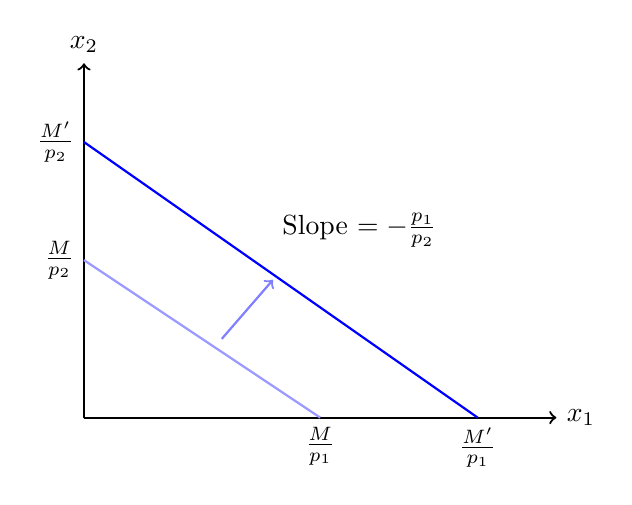
\begin{tikzpicture}[scale=0.5]
    % Axes
    \draw[->, thick] (0,0) -- (12,0) node[right] {$x_1$};
    \draw[->, thick] (0,0) -- (0,9) node[above] {$x_2$};

    % Initial budget line (income = M)
    \draw[thick, blue!40]
    (0,4) -- (6,0);

    % New budget line (income = M')
    \draw[thick, blue]
    (0,7) -- (10,0);

    % Intercepts
    \node[left] at (0,4) {$\frac{M}{p_2}$};
    \node[left] at (0,7) {$\frac{M'}{p_2}$};

    \node[below] at (6,0) {$\frac{M}{p_1}$};
    \node[below] at (10,0) {$\frac{M'}{p_1}$};

    % Slope annotation
    \node at (7,4.75) {Slope $= -\frac{p_1}{p_2}$};

    % Arrow indicating increase in income
    \draw[->, thick, blue!50]
    (3.5,2) -- (4.8,3.5);
    \end{tikzpicture}
    \end{center}
}


\slide{Decrease in Income}{
    Consider Example 1 again, wherein I go to Starbucks. Now, however, I go
    with \$5 instead of \$10. How does this impact the budget line?

    \begin{center}
    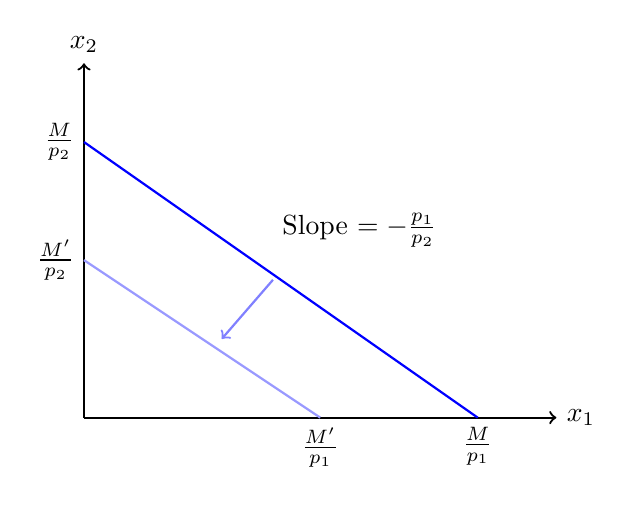
\begin{tikzpicture}[scale=0.5]
    % Axes
    \draw[->, thick] (0,0) -- (12,0) node[right] {$x_1$};
    \draw[->, thick] (0,0) -- (0,9) node[above] {$x_2$};

    % Initial budget line (income = M)
    \draw[thick, blue!40]
    (0,4) -- (6,0);

    % New budget line (income = M')
    \draw[thick, blue]
    (0,7) -- (10,0);

    % Intercepts
    \node[left] at (0,4) {$\frac{M'}{p_2}$};
    \node[left] at (0,7) {$\frac{M}{p_2}$};

    \node[below] at (6,0) {$\frac{M'}{p_1}$};
    \node[below] at (10,0) {$\frac{M}{p_1}$};

    % Slope annotation
    \node at (7,4.75) {Slope $= -\frac{p_1}{p_2}$};

    % Arrow indicating increase in income
    \draw[->, thick, blue!50]
    (4.8,3.5) -- (3.5,2);
    \end{tikzpicture}
    \end{center}
}


\subsection{Change in Prices}

\slide{Increase in Price of \texorpdfstring{\(x_1\)}{PDFstring}}{
    Consider Example 1 again, wherein I go to Starbucks. Now, however, the cookies
    cost \$2 instead of \$1. How does this impact the budget line?

    Initially the budget line was:
    \[x_1 + 2x_2 = 10 \;\; \Rightarrow \;\; x_2 = 5 - \frac{1}{2}x_1\]

    The budget line now becomes:
    \[2x_1 + 2x_2 = 10 \;\; \Rightarrow \;\; x_2 = 5 - x_1\]

    The absolute value of the slope has increased. This means that the line gets steeper.
}


\slide{Increase in Price of \texorpdfstring{\(x_1\)}{PDFstring}}{
\begin{center}
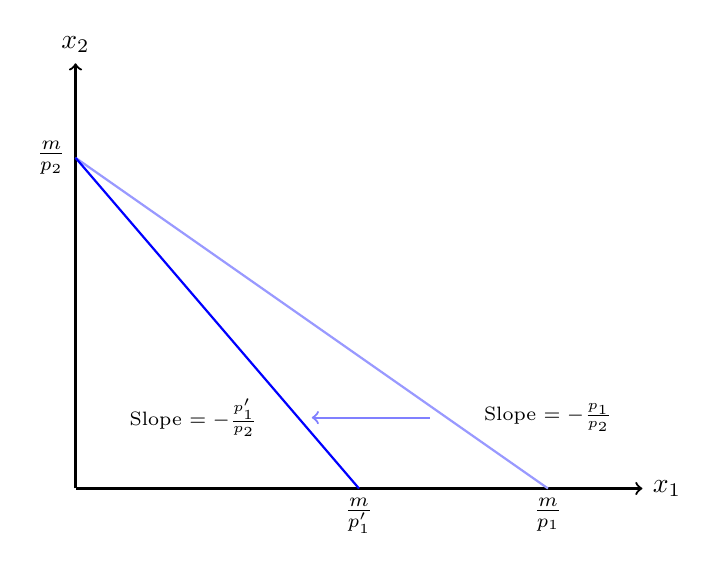
\begin{tikzpicture}[scale=0.6]
% Axes
\draw[->, thick] (0,0) -- (12,0) node[right] {$x_1$};
\draw[->, thick] (0,0) -- (0,9) node[above] {$x_2$};

% Original budget line (lower price p1)
\draw[thick, blue!40]
  (0,7) -- (10,0);

% New budget line (higher price p1')
\draw[thick, blue]
  (0,7) -- (6,0);

% Intercepts
\node[left] at (0,7) {$\frac{m}{p_2}$};

\node[below] at (10,0) {$\frac{m}{p_1}$};
\node[below] at (6,0) {$\frac{m}{p_1'}$};

% Slopes
\node[font=\scriptsize] at (10,1.5) {Slope $= -\frac{p_1}{p_2}$};
\node[font=\scriptsize] at (2.5,1.5) {Slope $= -\frac{p_1'}{p_2}$};

% Arrow indicating increase in price of x1
\draw[->, thick, blue!50]
(7.5,1.5) -- (5,1.5);
\end{tikzpicture}
\end{center}
}


\slide{Increase in Price of \texorpdfstring{\(x_2\)}{PDFstring}}{
    Consider Example 1 again, wherein I go to Starbucks. Now, however, the coffee
    cost \$4 instead of \$2. How does this impact the budget line?

    Initially the budget line was:
    \[x_1 + 2x_2 = 10 \quad \Rightarrow \quad x_2 = 5 - \frac{1}{2}x_1\]

    The budget line now becomes:
    \[x_1 + 4x_2 = 10 \quad \Rightarrow \quad x_2 = \frac{10}{4} - \frac{1}{4}x_1\]

    The absolute value of the slope has decreased. Therefore, the curve becomes flatter.
}


\slide{Increase in Price of \texorpdfstring{\(x_2\)}{PDFstring}}{
    \begin{center}
    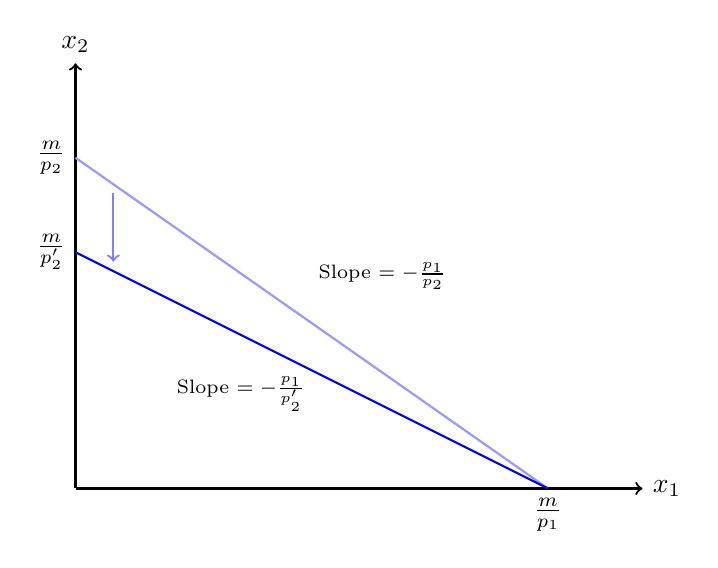
\begin{tikzpicture}[scale=0.6]
    % Axes
    \draw[->, thick] (0,0) -- (12,0) node[right] {$x_1$};
    \draw[->, thick] (0,0) -- (0,9) node[above] {$x_2$};

    % Original budget line (lower price p2)
    \draw[thick, blue!40]
    (0,7) -- (10,0);

    % New budget line (higher price p2')
    \draw[thick, blue]
    (0,5) -- (10,0);

    % Intercepts
    \node[left] at (0,7) {$\frac{m}{p_2}$};
    \node[left] at (0,5) {$\frac{m}{p_2'}$};

    \node[below] at (10,0) {$\frac{m}{p_1}$};

    % Slopes
    \node[font=\scriptsize] at (6.5,4.5) {Slope $= -\frac{p_1}{p_2}$};
    \node[font=\scriptsize] at (3.5,2) {Slope $= -\frac{p_1}{p_2'}$};
    
    % Arrow indicating increase in price of x2
    \draw[->, thick, blue!50]
    (0.8,6.25) -- (0.8,4.8);
    \end{tikzpicture}
    \end{center}
}


\slide{Decrease in Prices of \texorpdfstring{\(x_1\)}{PDFstring} and \texorpdfstring{\(x_2\)}{PDFstring}}{
    Consider Example 1 again, but now with initial prices \(p_1 = \$2\) and \(p_2 = \$2\).

    The budget line is:
    \[2x_1 + 2x_2 = 10\]

    \begin{center}
    \begin{tikzpicture}[scale=0.6]
    % Axes
    \draw[->] (0,0) -- (6,0) node[right] {$x_1$ (cookies)};
    \draw[->] (0,0) -- (0,6) node[above] {$x_2$ (coffee)};

    % Budget line: 2x1 + 2x2 = 10  =>  x2 = 5 - x1
    \draw[blue, thick] (0,5) -- (5,0);

    % Intercepts labels
    \node[left] at (0,5) {$5$};
    \node[below] at (5,0) {$5$};
    \end{tikzpicture}
    \end{center}
}


\slide{Decrease in Prices of \texorpdfstring{\(x_1\)}{PDFstring} and \texorpdfstring{\(x_2\)}{PDFstring}}{
    Now, consider a decrease in both prices from \$2 to \$1.

    The budget line, now, is:
    \[x_1 + x_2 = 10\]

    \begin{center}
    \begin{tikzpicture}[scale=0.375]
    % Axes
    \draw[->] (0,0) -- (12,0) node[right] {$x_1$ (cookies)};
    \draw[->] (0,0) -- (0,12) node[above] {$x_2$ (coffee)};

    % Budget line 1: 2x1 + 2x2 = 10  =>  x2 = 5 - x1
    \draw[blue, thick] (0,5) -- (5,0);
    % Budget line 2: x1 + x2 = 10  =>  x2 = 10 - x1
    \draw[blue, thick] (0,10) -- (10,0);

    % Intercepts labels
    \node[left] at (0,5) {$5$};
    \node[below] at (5,0) {$5$};
    \node[left] at (0,10) {$10$};
    \node[below] at (10,0) {$10$};

    % Arrow indicating decrease in prices
    \draw[->, thick, blue!50]
    (2.65,2.65) -- (4.9,4.8);
    \end{tikzpicture}
    \end{center}
}


\subsection{Taxation}

\slide{Specific Tax}{
    If the government imposes a \emph{specific tax}, this means that the consumer has to pay a certain amount to the government
    for each unit of a good they purchase.

    For example, in India, an excise duty of INR 19.90 (as of 10th April 2025) is paid per litre of petrol.

    How does a specific tax affect the budget line of a consumer?

    From a consumer's perspective, a tax is just like a higher price. Thus,
    a quantity tax of \(\$t\) per unit of good 1 changes the price of good 1
    from \(p_1\) to \(p_1 + t\). Therefore, the budget line gets steeper.
}


\slide{Ad-Valorem Tax}{
    A government can also impose a \emph{ad-valorem tax}, this means that the consumer has to pay a
    percentage amount of the retail value of a good as tax. Consequently, the amount of tax
    increases as the price of the good or service increases.

    For example, most states in the U.S.A. have sales taxes. If the sales tax is 6 percent, then a good that
    is priced at \$1 will actually sell for \$1.06.

    How does an ad-valorem tax affect the budget line of a consumer?

    The consumer has to pay \(p_1\) to the supplier and \(\tau p1\) to the government for each unit of the good
    so the total cost of the good to the consumer is \((1 + \tau)p1\). Therefore, the budget line gets steeper.
}


\subsection{Subsidy}


\slide{Specific Subsidy}{
    If, for example, the consumption of milk were subsidized, the government would pay some amount of money to each
    consumer of milk depending on the amount that consumer purchased (in reality, the price just decreases).
    
    If the subsidy is \(\$s\) per unit of consumption of good 1, then from the viewpoint of the consumer, the price of good 1 would be \(\$p_1 - \$s\).
    
    This would, therefore, make the budget line flatter.
}


\slide{Ad-valorem Subsidy}{
    If the government gives you back \$1 for every \$2 you donate to charity, then your donations to charity
    are being subsidized at a rate of 50 percent.
    
    In general, if the price of good 1 is \(p_1\) and good 1 is subject to an ad-valorem subsidy at rate
    \(\sigma\), then the actual price of good 1 facing the consumer is \((1 - \sigma)p1\).

    This would, therefore, make the budget line flatter.
}



\section{Summary}

\slide{Summary}{
\begin{itemize}
    \item The budget set consists of all bundles of goods that the consumer can
    afford at given prices and income. We will typically assume that there are
    only two goods, but this assumption is more general than it seems.

    \item The budget line is written as \(p_1x_1 +p_2x_2 = M\). It has a slope of \(-\frac{p_1}{p_2}\),
    a vertical intercept of \(\frac{m}{p_2}\), and a horizontal intercept of \(\frac{m}{p_1}\).

    \item Increasing income shifts the budget line outward, and decreasing income shift it inward.
    
    \item Increasing the price of good 1 makes the budget line steeper, and decreasing the price of good 1
    makes the budget line flatter.
    
    \item Increasing the price of good 2 makes the budget line flatter, and decreasing the price of good 2
    makes the budget line steeper.

    \item Taxes and subsidies change the slope of the budget line by
    changing the prices paid by the consumer.
\end{itemize}
}